
% This LaTeX was auto-generated from an M-file by MATLAB.
% To make changes, update the M-file and republish this document.

\documentclass{article}
\usepackage{graphicx}
\usepackage{color}

\sloppy
\definecolor{lightgray}{gray}{0.5}
\setlength{\parindent}{0pt}

\begin{document}

    
    
\section*{BiMat - Group Testing Use case}

\begin{par}
This use case will introduce the user to the functionalities about how to perform an statistical analysis of a group of bipartite networks (matrices). For doing that we will use the data from Flores et Al 2011. This data consist of 38 bipartite adjacency matrices of different sizes. Each matrix is named according to the first author paper from which it was extracted. We will perform an analysis of modularity and nestedness in the entire set.
\end{par} \vspace{1em}

\subsection*{Contents}

\begin{itemize}
\setlength{\itemsep}{-1ex}
   \item Add the source to the matlab path
   \item Creating a Group Testing object
   \item Perform an statististical analysis in the set of matrices
   \item Using a GroupTesting object to create your own plots
\end{itemize}


\subsection*{Add the source to the matlab path}

\begin{verbatim}
g = genpath('matlab'); addpath(g);
close all; %close all open figures
\end{verbatim}
\begin{par}
We need also to load the data from which we will be working on
\end{par} \vspace{1em}
\begin{verbatim}
load group_testing_data.mat;
\end{verbatim}


\subsection*{Creating a Group Testing object}

\begin{par}
If the number of random matrices and the null model are not assigned, 100 and AVERAGE are used as default. Here we will use 100 random matrices with the EQUIPROBABLE null model
\end{par} \vspace{1em}
\begin{verbatim}
gp = GroupTesting(grouptesting.matrices);    % Create the main object
\end{verbatim}

%\includegraphics [width=4in]{use_case_group_testing_01.eps}


\subsection*{Perform an statististical analysis in the set of matrices}

\begin{par}
Suppose that we are interested in calculating the modularity and nestedness using the NTC algorithm as Flores et Al 2011 did. In addition, following the approach of Flores et Al 2011, we want to use the equiprobable model as null model in our random networks. The way to perform this analysis is by running the next lines:
\end{par} \vspace{1em}
\begin{verbatim}
gp.replicates = 100; %How many random networks we want for each matrix
gp.null_model = @NullModels.EQUIPROBABLE; %Our Null model
gp.modul_class = @AdaptiveBrim; %Algorithm for modularity.
gp.do_temp = 1; % Perform NTC analysis (default)
gp.do_modul = 1; % Perform Modularity analysis (default)
gp.do_nest = 0; % Do not perform NODF analysis
gp.DoGroupTesting(); % Perform the analysis.
gp.names = grouptesting.name;
\end{verbatim}

        \color{lightgray} \begin{verbatim}Testing Matrix: 1 . . .
Testing Matrix: 2 . . .
Testing Matrix: 3 . . .
Testing Matrix: 4 . . .
Testing Matrix: 5 . . .
Testing Matrix: 6 . . .
Testing Matrix: 7 . . .
Testing Matrix: 8 . . .
Testing Matrix: 9 . . .
Testing Matrix: 10 . . .
Testing Matrix: 11 . . .
Testing Matrix: 12 . . .
Testing Matrix: 13 . . .
Testing Matrix: 14 . . .
Testing Matrix: 15 . . .
Testing Matrix: 16 . . .
Testing Matrix: 17 . . .
Testing Matrix: 18 . . .
Testing Matrix: 19 . . .
Testing Matrix: 20 . . .
Testing Matrix: 21 . . .
Testing Matrix: 22 . . .
Testing Matrix: 23 . . .
Testing Matrix: 24 . . .
Testing Matrix: 25 . . .
Testing Matrix: 26 . . .
Testing Matrix: 27 . . .
Testing Matrix: 28 . . .
Testing Matrix: 29 . . .
Testing Matrix: 30 . . .
Testing Matrix: 31 . . .
Testing Matrix: 32 . . .
Testing Matrix: 33 . . .
Testing Matrix: 34 . . .
Testing Matrix: 35 . . .
Testing Matrix: 36 . . .
Testing Matrix: 37 . . .
Testing Matrix: 38 . . .
\end{verbatim} \color{black}
    \begin{par}
Notice that \texttt{DoGroupTesting} method prints informatino about the current networks that is being analyzed, such that the user will know at every moment the current status of the analysis. After the analysis is finished a simple statistical measure to say that a matrix is nested and/or modular is to chose a two tail p-value = 0.05 as Flores et al 2011 did. Therefore, the next lines of code will show how many matrices are found nested and/or modular
\end{par} \vspace{1em}
\begin{verbatim}
fprintf('Number of nested matrices: %i\n',sum(gp.tempvals.percent >= 97.5));
fprintf('Number of modular matrices: %i\n',sum(gp.qb_vals.percent >= 97.5));
\end{verbatim}

        \color{lightgray} \begin{verbatim}Number of nested matrices: 29
Number of modular matrices: 6
\end{verbatim} \color{black}
    \begin{par}
We can also show the entire set of results by calling:
\end{par} \vspace{1em}
\begin{verbatim}
gp.PrintResults();
\end{verbatim}

        \color{lightgray} \begin{verbatim}Network,      Qb, Qb mean,Qb z-score,Qb percent,    NTC,NTC mean,NTC z-score,NTC percent
      1, 0.30992, 0.27504,    1.1839,        88,0.65025,  0.6665,   -0.16359,         46
      2,  0.2144,  0.3912,   -5.3337,         0,0.80601, 0.69599,      1.398,         92
      3, 0.17556, 0.24949,   -2.4165,         0,0.99985, 0.65143,     4.2546,        100
      4, 0.22449, 0.40398,   -3.3133,         0, 0.9352, 0.75818,     1.8262,         98
      5, 0.25652, 0.30693,   -3.1638,         0,0.94524, 0.55571,     6.3094,        100
      6,  0.2699, 0.50311,   -3.9409,         0,0.82486, 0.79025,    0.44245,         65
      7, 0.21403, 0.32558,    -3.915,         0,0.98175, 0.64499,     4.1166,        100
      8,   0.174, 0.24764,   -8.2717,         0,0.79747, 0.41325,      8.298,        100
      9, 0.21847, 0.34734,  -10.5782,         0,0.85665, 0.53498,     7.1639,        100
     10, 0.29191, 0.27905,   0.63395,        77,0.62778, 0.57744,    0.62582,         73
     11, 0.24033, 0.38291,   -6.3425,         0,0.82975, 0.63798,      2.548,        100
     12,  0.4821, 0.40885,    2.8292,       100,0.86341, 0.64601,     2.7081,        100
     13, 0.32099, 0.48247,   -2.0874,         1,0.92493, 0.88012,    0.65538,         68
     14, 0.31667, 0.34527,  -0.87022,        20,0.76809, 0.56685,       4.01,        100
     15, 0.20023, 0.26569,   -6.9718,         0,0.72107,  0.4401,     6.0606,        100
     16, 0.18956, 0.19473,   -1.0706,        15,0.83344, 0.33072,    16.5544,        100
     17,0.045608,0.050704,    -1.907,         0,0.99893, 0.84626,     3.9775,        100
     18,  0.1231, 0.15641,   -4.3656,         0,0.90103, 0.61259,     3.6611,        100
     19,       0, 0.27955,   -8.7977,         0,0.63018, 0.63717,  -0.094411,         51
     20, 0.31027,  0.4648,   -6.6651,         0,0.85738, 0.64139,     5.0965,        100
     21, 0.19136, 0.38985,    -4.279,         0,0.97793, 0.72472,     2.2901,        100
     22, 0.22015, 0.17924,    8.0624,       100,0.98062, 0.35562,     17.595,        100
     23, 0.08406, 0.10171,   -5.4743,         0,0.98762, 0.61385,     5.7749,        100
     24,  0.4102, 0.34771,    3.8622,       100,0.70825,  0.5598,     2.5713,         99
     25, 0.14966, 0.19785,   -2.0806,         2,0.85489, 0.77844,     0.7644,         77
     26,0.053624, 0.10053,   -8.0929,         0,0.87661, 0.61226,      5.734,        100
     27, 0.20209,  0.2118,   -1.0999,        15,0.83542, 0.43909,    12.8152,        100
     28, 0.37025, 0.38953,   -1.3666,         6,0.80778, 0.59887,     4.4616,        100
     29, 0.37622, 0.26297,   10.2184,       100,0.64478, 0.48073,     2.7071,        100
     30, 0.33347,  0.3352,  -0.10286,        50,0.93098, 0.55137,     6.3186,        100
     31, 0.22893, 0.46138,    -5.965,         0,0.97517,  0.6977,     4.1492,        100
     32, 0.18341, 0.14642,    9.5873,       100,0.92846, 0.36512,    15.2961,        100
     33, 0.39459, 0.39213,   0.19076,        58,0.78705, 0.60728,     4.5664,        100
     34,  0.4876, 0.53545,  -0.57811,        28,0.90565, 0.87035,     0.4289,         58
     35,0.084203,0.084698,  -0.18344,        44,0.94646, 0.69432,     4.1231,        100
     36, 0.61983, 0.63421,  -0.17118,        39,0.98783, 0.94318,     1.3557,        100
     37, 0.21828, 0.27477,   -7.0181,         0,0.88695, 0.41636,    15.0226,        100
     38, 0.68222, 0.57676,    3.2272,       100,0.83338, 0.82711,    0.19745,         50
\end{verbatim} \color{black}
    

\subsection*{Using a GroupTesting object to create your own plots}

\begin{par}
We can use a GroupTesting object (gp in this case) to create specific plots. Suppose we are interested in plotting all the matrices in modular sorting, such that the lables in the matrix are in red if the matrix is modular and in blue if it is antimodular. A simple script for performing this task will be:
\end{par} \vspace{1em}
\begin{verbatim}
n_rows = 5;
n_cols = 8;
modular_indices = gp.qb_vals.percent >= 97.5;
no_modular_indices = gp.qb_vals.percent <= 2.5;
figure(1);
for i = 1:gp.n_networks
    subplot(n_rows, n_cols, i);
    gp.networks{i}.plotter.use_labels = 0; %Do not show row/column labels
    gp.networks{i}.plotter.use_isocline = 0; %No isocline inside modules
    gp.networks{i}.plotter.PlotModularMatrix();
    col = 'black'; % Color for not significance
    if(modular_indices(i) == 1) % Color for significant modularity
        col = 'red';
    elseif(no_modular_indices(i) == 1) % Color for significant antimodularity
        col = 'blue';
    end
    title(gp.names{i},'Color',col, 'FontSize',10);
end
set(gcf,'Position', [148         213        1142         746]);
\end{verbatim}

%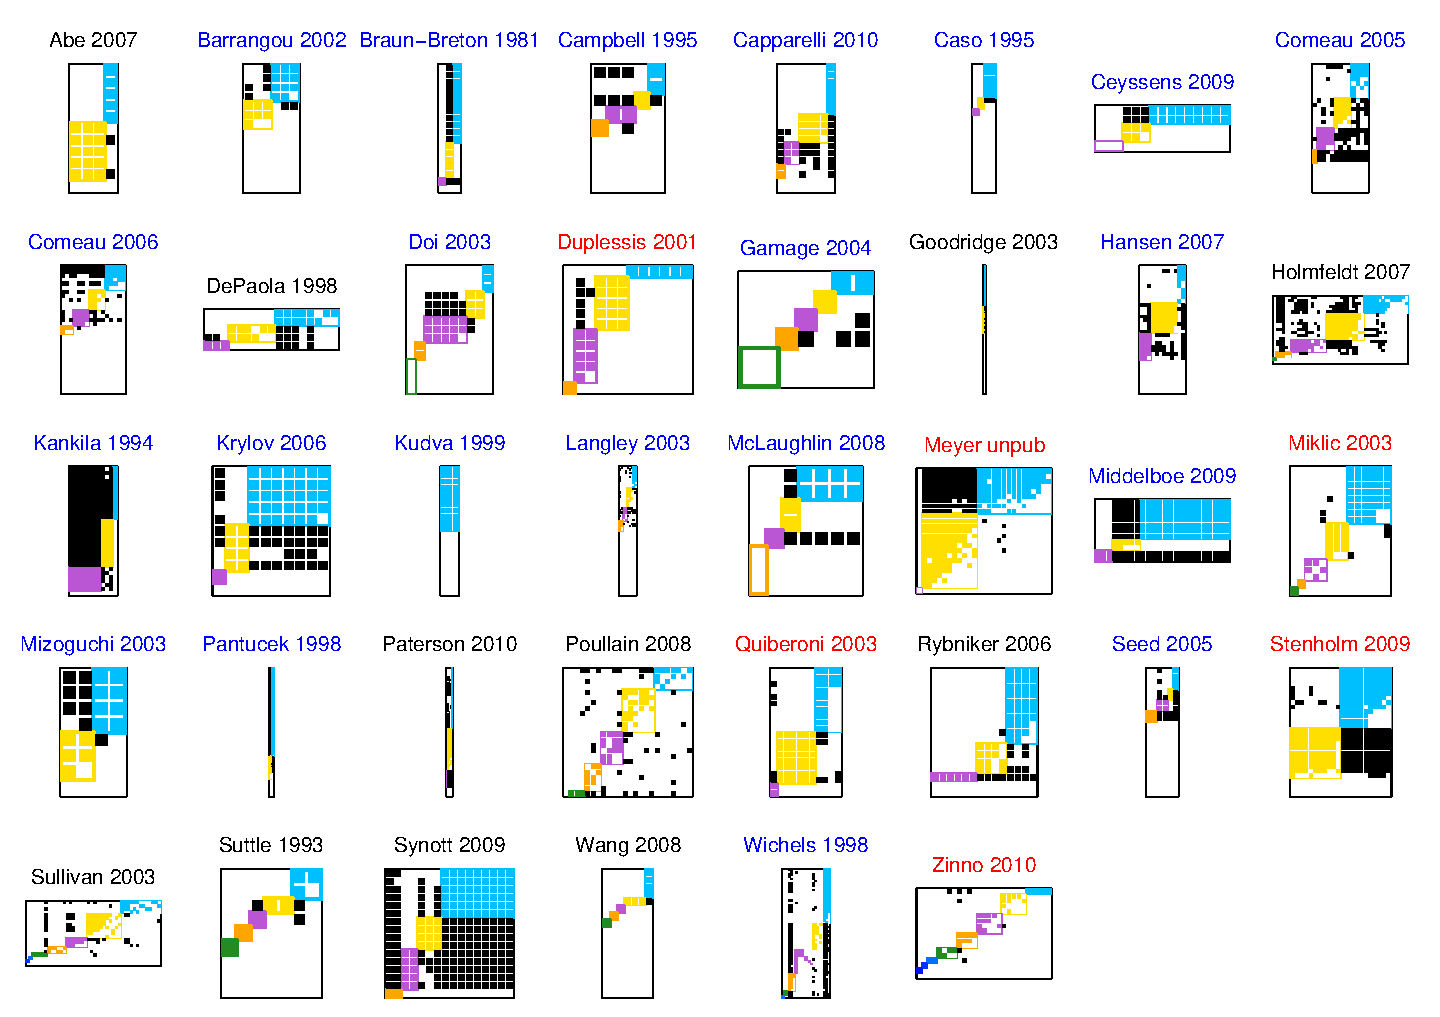
\includegraphics [width=4in]{use_case_group_testing_02.eps}
\begin{par}
We may want to create a plot that compare the values of the networks with the random values of the null model. The next lines will show how to create such plot for the case of the NTC results
\end{par} \vspace{1em}
\begin{verbatim}
ntc_vals = gp.tempvals.value;
[~,sorted_indexes] = sort(ntc_vals); % I will plot in increasing NTC value

%Get random values and sort according to sorted_indexes
ntc_vals = ntc_vals(sorted_indexes);
mean_random_vals = gp.tempvals.mean(sorted_indexes);
random_values = gp.tempvals.random_values; %variable already sorted in rows
random_values = random_values(sorted_indexes,:); %sort in rows
names = gp.names(sorted_indexes);

%Find the limits of the error bars using two tail p-value=0.05
sup_bound = random_values(:,round(gp.replicates * 0.975));
low_bound = random_values(:,round(gp.replicates * 0.025));

%Plot the data of the real matrices
figure(2);
plot(1:gp.n_networks, ntc_vals,'o','MarkerFaceColor','red','MarkerEdgeColor','red');
hold on;
%Plot the data of the random values
errorbar(1:gp.n_networks, mean_random_vals, mean_random_vals - low_bound, ...,
    sup_bound - mean_random_vals, 'o','MarkerFaceColor','white','MarkerEdgeColor','black');
hold off;

%Write the labels
set(gca,'xticklabel',[]);
for i=1:gp.n_networks
    tmph=text(i,-0.01,names(i));
    set(tmph,'HorizontalAlignment','right');
    set(tmph,'rotation',90);
    set(tmph,'fontsize',10);
end

%Labels in title, y-axis and legends
tmplh = legend('Measured modularity','Random expectation',1,'Location','NorthWest');
legend('boxoff')
title('Nestedness in Bacteria-Phage Networks','fontsize',20);
ylabel('Nestedness (NTC)','fontsize',16);

%Give format to the matrix
xlim([1 1+gp.n_networks]);
ylim([0 1]);

%Give appropiate size to the figure window
set(gcf,'Position',[91   135   859   505]);
set(gca,'Units','pixels');
set(gcf,'Position', [91   135   859   505+150])
apos = get(gca,'position');
apos(2) = apos(2) + 82;
set(gca,'position',apos);
set(gcf,'position',[91   135   859   596]);
\end{verbatim}

%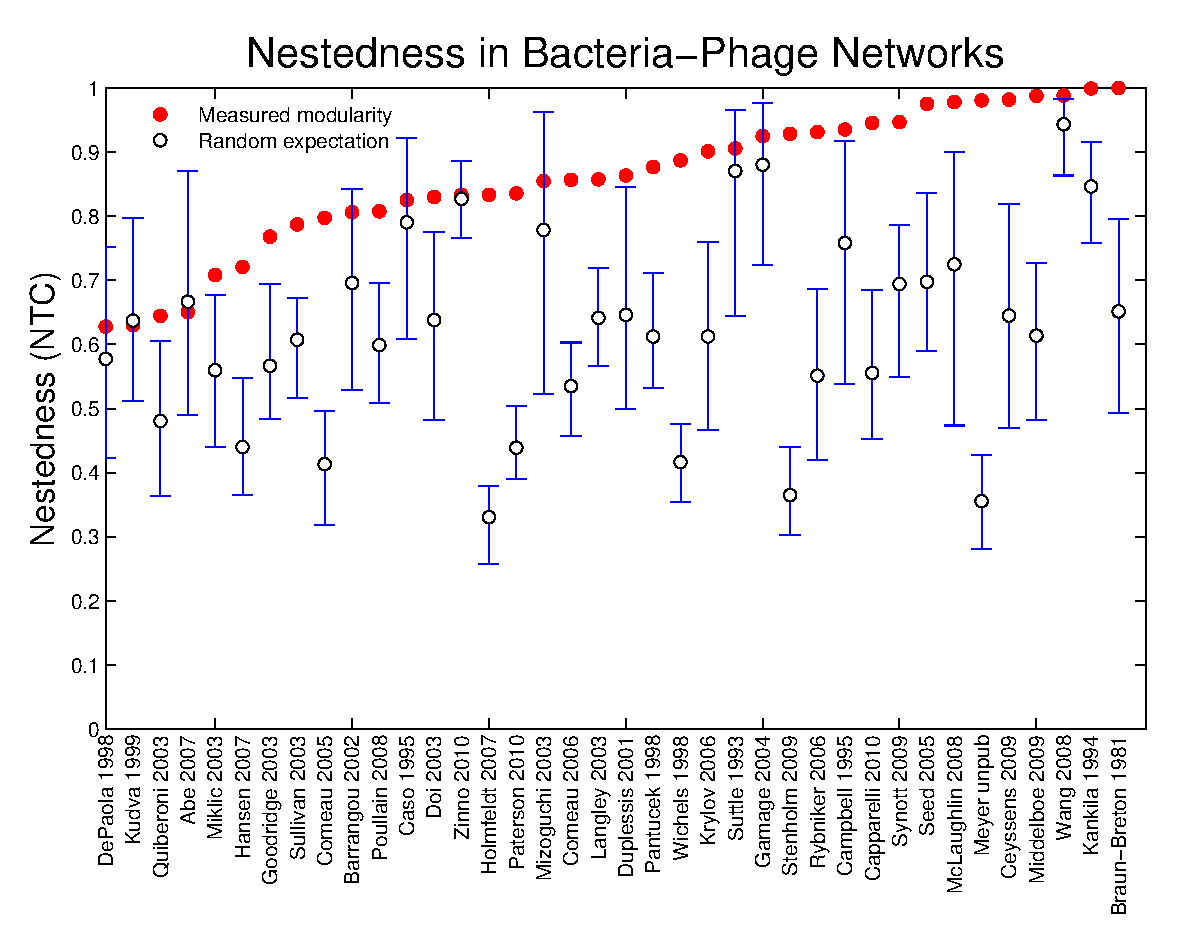
\includegraphics [width=4in]{use_case_group_testing_03.eps}



\end{document}
    
